\documentclass[12pt,a4paper]{article}
\usepackage[utf8]{inputenc}
\usepackage[german]{babel}
\usepackage[T1]{fontenc}
\usepackage{times}
\usepackage{graphicx}
\usepackage{url}
\usepackage{color}
\usepackage{setspace}
\usepackage{xcolor}
\usepackage{enumerate}
\usepackage{amsmath}
\usepackage{amsfonts}
\usepackage{subfigure}
\usepackage{amssymb}
\usepackage{float}
\usepackage{stix}
\title{Machine Learning 1}
\author{Henrik Tscherny}
\DeclareMathOperator*{\argmin}{argmin}
\DeclareMathOperator*{\argmax}{argmax}
\newcommand{\nl}{\\[0.1cm]}
\newcommand{\red}[1]{\textcolor{red} {#1}}
\newcommand{\blue}[1]{\textcolor{blue} {#1}}


% \pagecolor[rgb]{0,0,0}
% \color[rgb]{0,0.7,0}

\begin{document}
\maketitle
\tableofcontents

\section{Supervised learning}
Ziel: Finde in einer Funktionsfamilie, z.B. lineare Funktionen, eine Funktion z.B. $f = 5x+3$ welche eine gewichtete Summe über input-output-Paaren minimiert, dabei sollte die Funktion die gegebenen Daten bestmöglich beschreiben ohne dabei zu komplex zu sein\\

Beispiel:
\begin{itemize}
\item $g: \Theta \rightarrow Y^X$ -> Ordnet jeder Messung zu ob gesund oder krank\\
$g_{\theta}(x_s) = \begin{cases} 0, & \displaystyle\sum_{j=1}^n \Theta_j x_j > 0 \\ 1, & sonnst \end{cases}$, für ein Sample $x_s\in \mathbb{R}^m$
\begin{itemize}
\item $x \in X=\mathbb{R}^n$: Inputs ->  Messung mit m Messpunkten
\item $y \in Y = \{0,1\}$: Labels -> gesund = 1, krank = 0
\item $\theta \in \Theta = \mathbb{R}^n$: Parameter -> z.B. Koeffizienten einer linearen Funktion
\end{itemize}
\end{itemize}

Die Qualität einer gelernten Funktion kann u.a. durch folgende Größen beschrieben werden:
\begin{itemize}
\item \textbf{Accuracy} (Verhältnis der korrekten Voraussagen zur Gesamtanzahl)\nl
$\frac{L(0,0)+L(1,1)}{|S|}$ 
\item \textbf{Error ratio} (Verhältnis der falschen Voraussagen zu Gesamtanzahl)\nl
$\frac{L(0,1)+L(0,1)}{|S|}$
\item \textbf{Precision} (Von den positiv getesteten, wie viele sind tatsächlich positiv) False-Positive-Rate\nl
$\frac{L(1,1)}{L(1,0)+L(1,1)}$
\item \textbf{Recall/Sensitivity} (Von den tatsächlich positiven, wie viele wurden tatsächlich positiv getestet) False-Negative-Rate\nl
$\frac{L(1,1)}{L(0,1)+L(1,1)}$
\end{itemize}

\subsection{Formal}
Optimieren einer Funktionsfamilie $g: \Theta \rightarrow \{0,1\}^X$, damit dies einfacher ist, optimieren einer Relaxation $f: \Theta \rightarrow \mathbb{R}^X$. Sei L eine Loss-function $L: \mathbb{R} \times \{0,1\} \rightarrow \mathbb{R}_0^+$ welche g im Bezug zu f definiert.\nl
$\displaystyle \forall \theta \in \Theta \forall x \in X: g_\theta(x) \in \argmin_{\hat{y} \in \{0,1\}} L(f_\theta(x),\hat{y})$\\
Bsp. Loss-function:\nl
\textbf{0-1-Loss}:
$\displaystyle L=\begin{cases} 0,& sample=label\\ 1, & sonnst \end{cases}$, der Loss ist 0\% wenn das Label stimmt\nl

Definiere des Weiteren:
\begin{itemize}
\item S: Samples
\item X: Attributspace
\item $x: S\rightarrow X$: bildet ein konkretes Sample mit seinen Attributen ab
\item $y: S\rightarrow \{0,1\}$ gibt einem konkreten Sample ein Label
\end{itemize}

Das Tupel $T=(S,X,x)$ nennt man \textbf{unlabled data}\\
Das Tupel $T=(S,X,x,y)$ nennt man \textbf{labeled data}\nl

Damit die Komplexität der zu lernenden Funktion begrenzt wird, führen wir zusätzlich noch einen \textbf{Regularizer}. Komplexität kann in diesem Fall z.B. die Anzahl der Koeffizienten oder die Länge einer Formel bemessen werden. Der Einfluss des Regularizers wird durch einen Parameter $\lambda$ gesteuert\nl
$R: \Theta \rightarrow \mathbb{R}_0^+$ und $\lambda\in\mathbb{R}_0^+$\nl
Das \textbf{supervised learning problem} kann dann wie folgt formuliert werden:\nl
$\displaystyle \inf_{\theta\in\Theta} \; \lambda R(\theta) + \frac{1}{|S|} \sum_{s\in S} L(f_\theta (x_s), y_s)$
\begin{itemize}
\item der Regularizer wird durch $\lambda$ gewichtet
\item es wird die Summe der individuellen Loss-Werte minimiert
\item die Loss-Summe wird über die Anzahl der Samples Normalisiert, das macht man, damit man lediglich die Parameter übertragen muss, wenn man das Model weitergibt
\item Da der Regularizer zum Gesamtloss addiert wird, wird versucht diesen Term ebenfalls möglichst klein zu halten
\end{itemize}
Das \textbf{separation problem} ist definiert durch:\nl
$\displaystyle \inf_{\theta \in \Theta} R(\theta) \\ \forall s\in S: f_\theta(x_s) = y_s$
\begin{itemize}
\item finden des minimalen Regularizers
\item alle Daten sind korrekt gelabeled
\end{itemize}
Das \textbf{bounded separability problem} lautet:\nl
$R(\theta) \leq m \\ \forall s\in S: \; f_\theta(x_s) = y_s$
\begin{itemize}
\item finden eines Regularizers welcher die Komplexität für jeden Parameter unter einer Schranke m hält
\end{itemize}
Das \textbf{inference problem} (Anwenden des trainierten Modells) kann nun wie folgt formuliert werden:\nl
$\displaystyle \min_{y'\in \{0,1\}^S}\sum_{s\in S}L(\hat{f}(x_s),y'_s)$
$\displaystyle = \sum_{s\in S} \min_{y'\in \{0, 1\}^S} L(\hat{f}(x_s),y'_s)$

\section{Disjunktive Normalformen (DNF'S)}
Probleme können ebenfalls als logische Gleichungen interpretiert werden, diese Gleichungen können dann in eine DNF (Mit oder verbundene und-Terme) umgeformt werden.
\subsection{Formal}
\begin{itemize}
\item $\Gamma = \{(V_0, V_1) \in 2^V \times 2^V \vert V_0 \cap V_1 = \emptyset\}$\nl
Jede Variable kann entweder negiert oder nicht-negiert vorkommen
\item $\Theta = 2^\Gamma$
\item $\displaystyle \forall x \in \{0,1\}^V: \; f_\theta(x)= \bigwedge_{(V_0,V_1)\in\theta}\prod_{v\in V_0} (1-x_v) \prod_{v\in V_1} x_v$\nl
Definition einer DNF, veroderte negierte und nicht-negierte Variablen
\end{itemize}

\textbf{Beispiel}
$\{(\emptyset,  \{v_1, v_2\}), (\{v_1\}\{v_3\})\} = \theta \in \Theta \; \rightarrow f_\theta(x) = x_{v_1}x_{v_2} \lor (1-x_{v_1})x_{v_3}$\nl

Des Weiteren können Regularizer für DNF's definiert wenn, um deren Komplexität zu bemessen:
\begin{itemize}
\item $\displaystyle R_d(\theta) = \max_{(V_0,V_1)\in\theta} (|V_0| + |V_1|)$\nl
Tiefe der Formel, e.g. Anzahl der Variablen des längsten und-Terms
\item $\displaystyle R_l(\theta) = \sum_{(V_0,V_1)\in\theta} (|V_0| + |V_1|)$\nl
Länge der Formel, e.g. Gesamtanzahl der Variablen in der Gesamtformel (auch doppelte zählen)
\end{itemize}
\textbf{Beispiel} $\theta = \{(\emptyset, \{0\}),\,(\{0\},\,\{3\}),(\{0,3\},\{1,2\}))\}\\
\rightarrow f_\theta(x) = x_0 \lor (1-x_0)x_3\lor (1-x_0)(1-x_3)x_1 x_2 \rightarrow R_l(\theta) = 7 ,\; R_d(\theta)=4$\nl


Das \textbf{Supervised learning problem of DNF's} kann wie folgt formuliert werden:\nl
$\displaystyle \min_{\theta \in \Theta} R(\theta) \\ \forall s\in S: f_\theta(x_s) = y_s$
\begin{itemize}
\item Der Unterschied ist lediglich, dass ein $\min$ statt eines $\inf$ benutzt wird\
\item min: kleinstes Element einer Menge und muss in der Menge selbst liegen
\item inf: größte untere Schranke, muss nicht in der Menge selbst liegen, es müssen nur alle Elemente kleiner sein
Des Weiteren erhält man das \textbf{bounded depth/length DNF Problem} indem man den Regularizer aus dem bounded sparability problem mit $R_d/R_l$ austauscht
\end{itemize}

\textbf{Das bounded length/depth DNF problem ist NP-hard}\\
Beweis durch Reduktion des set cover problems auf das bounded length/depth DNF problem (Haussler):\nl
Was ist ein Set-Cover:
\begin{itemize}
\item Sei S eine eine Menge
\item Sei $\Sigma \subseteq 2^S, \; \emptyset\not\in\Sigma$ ein Cover, gdw. $\displaystyle \bigcup_{U\in\Sigma} U = S$
\item $m\in\mathbb{N}$
\item Die Entscheidung ob ein $\Sigma' \subseteq \Sigma$ existiert, s.d. $|\Sigma'|\leq m$ nennt man das \textbf{set cover problem} (S, $\Sigma$, m)
\end{itemize}
Beispiel:\\
Sei $S = \{1,2, 3, 4, 5, 6\}$, dann ist ein mögliches Cover $\Sigma = \{\{1, 2, 3\},\{4, 5, 6\}\}$ (m=2)

\subsection{Beweis der NP-hardness von set-cover}
Wir zeigen das set-cover NP-hard ist indem wir es auf bounded length/depth DNF reduzieren (Haussler)
\begin{itemize}
\item Sei $(S', \Sigma, m)$ eine Instanz von set-cover
\item Definiere nun \textbf{Haussler data} $(S, X, x, y)$ s.d.:
\begin{itemize}
\item $S = S' \cup \{\red{1}\}$, wir fügen S ein spezielles distinktes Element \red{1} hinzu
\item $X = \{0, 1\}^\Sigma$
\item wir definieren uns eine Funktion welche angibt ob ein Element in einer Menge vorkommt wie folgt:\\
$\displaystyle \forall s \in S' \, \forall \sigma \in \Sigma: \; x_s(\sigma) = \begin{cases}0, \; s\in \sigma \\ 1, \; \text{otherwise}\end{cases}$\\
Beispiel:
\begin{itemize}
\item $S = S' \cup \{\red{1}\} = \{2, 3\} \cup \{\red{1}\} = \{\red{1}, 2, 3\}$
\item $\Sigma = \{\{2\},...,\{1, 2\},...,\{2, 3\}\}$
\item $x_2(\{2, 3\}) = 0, \; x_3(\{2\}) = 1$
\end{itemize}
\item $x_{\red{1}} = 1^\Sigma$, das spezielle Element kommt nirgends vor
\item $y_{\red{1}} = 1$ und $\forall s \in S': y_s = 0$, wir definieren das label das  spezielle Element 1, für alle anderen 0
\end{itemize}
\item z.z. Lemma: $\displaystyle \bigcup_{\sigma \in \Sigma'} = S' \Leftrightarrow \forall s\in S' : \prod_{\sigma\in\Sigma'}x_s(\sigma) = 0$\\
set-cover kann umgeschrieben werden in ein Produkt mittel der Funktion $x_s$ (das Produkt verhält sich wie ein logisches UND)
\begin{itemize}
\item $\displaystyle \bigcup_{\sigma \in \Sigma'} = S'$
\item $\Leftrightarrow \forall s\in S' \, \exists \sigma \in \Sigma': \; s\in\sigma$, für jedes Sample ex. eine TM mit diesem Sample
\item $\Leftrightarrow$ für dieses Sample gilt somit $x_s(\sigma) = 0$, d.h. es ex. ein Sample für die die Funktion 0 ist
\item $\Leftrightarrow$ Existenz kann mittel des logischen UND's repräsentiert werden\\
$\displaystyle \forall s\in\Sigma':\; \prod_{\sigma\in\Sigma'}x_s(\sigma)=0$
\end{itemize}
\item \textbf{Beweis NP-hardness}:\\
z.z.: $\exists\, \Sigma' \subseteq \Sigma$ von $S'$ mit $|\Sigma'|\leq m$ $\Leftrightarrow \exists\, \theta\in\Theta: R(\theta) \leq m$ und\\
$\forall s \in S: \, f_\theta(x_s)=y_s$\\
d.h., es ex. ein Lösung von set-cover mit bound m gdw. es Parameter $\theta$ mit Komplexität $\leq$ m gibt und alle Samples korrekt inferred werden

\item ($\Rightarrow$)
\begin{itemize}
\item Sei $\Sigma' \subseteq \Sigma$ ein Cover von S mit $\Sigma'|\leq m$
\item Sei $V_0 = \emptyset, \; V_1=\Sigma'$, d.h wir definieren das Cover als Menge der nicht-negierten Variablen einer DNF
\item $\displaystyle \forall x' \in X:\; f_\theta(x')=\prod_{\sigma\in\Sigma'} x'(\sigma),\;$ (DNF mit nur positiven Variablen)
\item siehe Lemma muss dieses Produkt gleich 0 sein $\forall s \in S':\;f(x_s)=0$
\item Laut Definition gilt zudem $f(1^\Sigma)=1$
\item daraus folgt, dass alle Daten richtig gelabelt wurden\\ $\forall s\in S': f(x_s)=y_s$
\item Da wir $V_1 = \Sigma'$ und $V_0 = \emptyset$ gesetzt haben, ist der Regularizer auch gleich $R(\theta)= |\Sigma'| \leq m$
\end{itemize}
\item ($\Leftarrow$)
\begin{itemize}
\item Sei $\theta \in \Theta$ s.d. alle Daten richtig inferred werden und $R(\theta) \leq m$
\item TODO: verstehe Beh. am Anfang
\item TODO: what is going on here ?
\end{itemize}
\end{itemize}

\section{BTD's}
\subsection{Formal}
Ein V-variant BTD kann als Tupel $\theta = (V,Y,D,D',d*,E,\delta,v,y)$ wie folgt dargestellt werden
\begin{itemize}
\item eine Menge von Variablen: $V \neq \emptyset$
\item eine Menge von Werten: $Y \neq \emptyset$
\item einem (Sub)Tree $(D\cup D', E)$
\begin{itemize}
\item eine Menge von Inner-Nodes: $D$
\item eine Menge von Leaves: $D'$
\item ein Wurzelknoten: $d^*$
\item Kanten: $E$
\end{itemize}
\item Kantenfunktion: $\delta: E \rightarrow \{0,1\}$
\begin{itemize}
\item Jede Inner-Node $(d\in D)$ hat genau 2 ausgehende Kanten
\item $e=(d,d')$ mit $\delta(e) = 0$
\item $e'=(d,d'')$ mit $\delta(e') = 1$
\end{itemize}
\item Variablenfunktion: $v:D\rightarrow V$, Weißt Inner-Nodes eine Variable zu 
\item Wertefunktion: $y:D'\rightarrow Y$, Weißt Blättern einen Wert zu
\end{itemize}
Des Weiteren definieren wir noch den \textbf{Nachfolgeknoten von d}, wenn wir den \textbf{Weg j} nehmen als $\mathbf{d_{\downarrow j}}$

\begin{figure}[H]
\subfigure[BTD]{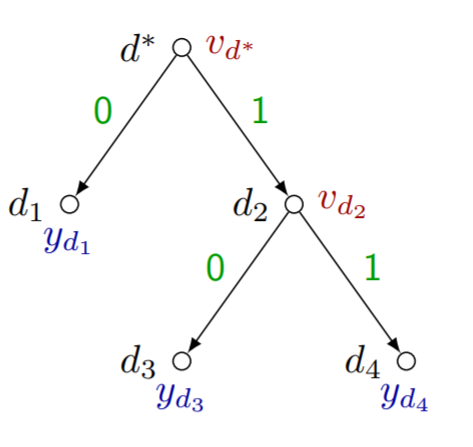
\includegraphics[width=.43\textwidth]{./resources/btd.png}}
\subfigure[$d_\downarrow$]{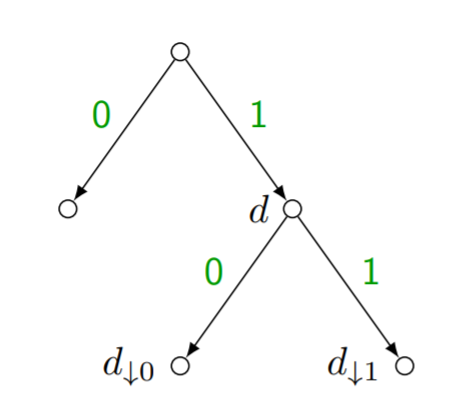
\includegraphics[width=.45\textwidth]{./resources/btd_down.png}}
\end{figure}

Für den Subtree von $\theta$ mit der Wurzel d schreibt man $\theta[d]$\\
Jeder Subtree von $\theta$ mit Wurzel d ist selbst wieder ein V-variante Y-valued BTD\nl
Für jeden BTD $\theta$ lässt sich ebenfalls wieder eine Funktion $f_\theta$ wie folgt definieren: $f_\theta : \{0, 1\}^V \rightarrow Y,\; \forall x\in \{0,1\}^V$
$\displaystyle f_\theta(x) = \begin{cases} y(d^*), & D = \emptyset\\
f_{\theta [d^*_{\downarrow 0}]}(x), & D \neq \emptyset \land x_v(d^*) = 0\\
f_{\theta [d^*_{\downarrow 1}]}(x), & D \neq \emptyset \land x_v(d^*) = 1\end{cases}$
Diese Funktion löst den BTD nacheinander rekursiv auf und betrachtet dabei in jeder Iteration einen kleineren Sub-BTD, bis dieser nur noch aus einen einzelnen Knoten besteht
\begin{itemize}
\item ist der BTD leer, d.h. es gibt nur eine Node, d.h. die Wurzel ist zugleich ein Leave, dann nehme den Wert davon, Ende der Rekursion
\item ist der Baum nicht leer, dann überprüfe die Variable an der Wurzel $x_v(d^*)$ und dann:
\begin{itemize}
\item nimm den linken Sub-BTD (0-Pfad) falls $x_v = 0$
\item nimm den rechten Sub-BTD (1-Pfad) falls $x_v = 1$
\end{itemize}
\item Fahre mit dem Sub-BTD rekursiv weiter fort
\end{itemize}
Wie auch Für DNF's kann für BTD's ein Regularizer angegeben werden, dieser gibt die \textbf{Tiefe} des BTD's an und ist ebenfalls rekursiv definiert:\nl
$\displaystyle R(\theta) = \begin{cases}0, & D = \emptyset \\
1+\max\{R(\theta[d^*_{\downarrow 0}]), R(\theta[d^*_{\downarrow 1}])\}, & \text{else}\end{cases}$\nl
Quasi, \textbf{Wie lang ist der längste Pfad im Baum, beginnend von der Wurzel}\nl
Ebenfalls kann für BTD's analog das supervised learning bzw. das bounded depth BTD problem definiert werden

\subsection{NP-hard Beweis}
Dazu reduzieren wir das das NP-schwere \textbf{exact cover by 3-sets} Problem auf das \textbf{bounded depth BTD} Problem\nl
Ein \textbf{exact cover} ist ein cover bei welchem alle Elemente paarweise disjunkt sind\nl
\textbf{exact cover by 3-sets problem}:
\begin{itemize}
\item Sei S eine Menge
\item Sei $\Sigma \subseteq 2^S \setminus \{\emptyset\}$
\item Lässt sich ein $\Sigma' \subseteq \Sigma$ finden, s.d. es nur Mengen der Größe 3 gibt, welche S exakt überdecken (dazu muss S natürlich ein vielfaches von 3 Elemente enthalten)
\red{Warum müssen es 3 sein geht doch auch mit einer anderen Zahl ?}
\end{itemize}
Definitionen:
\begin{itemize}
\item Sei $(S',\Sigma)$ eine Instanz des exact cover by 3-sets problem
\item Sei $|S'| = 3n$ mit $n\in\mathbb{N}$
\item Wir konstruieren eine Instanz des m-bounded depth BTD Problems wie folgt:
\begin{itemize}
\item Sei $V=\Sigma$, die Variablen des BTD's sind die möglichen Mengen welche zum Überdecken benutzt werden können
\item $S=S'\cup\{\red{0}\}$, wir fügen ein distinktes Element \red{0} hinzu
\item Sei $x:S\rightarrow \{0,1\}^\Sigma$, eine Funktion welche angibt ob ein Element in einer Menge vorkommt (analog wie bei DNF, nur invertiert)
\item Das spezielle Element \red{0} kommt dabei nirgends vor, d.h. $x_{\red{0}} = 0$
\item $y:S\rightarrow \{0,1\}$, weißt dem speziellen Element \red{0} das Label 0 zu, allen anderen das Label 1, d.h. $y_{\red{0}} = 0$
\item $m=n$
\end{itemize}
\end{itemize}
Wir zeigen nun, dass es ein exact cover gibt gdw. das bounded BTD problem eine Lösung hat
Beweis:
\begin{itemize}
\item ($\Rightarrow$)
\begin{itemize}
\item Sei $\Sigma' \subseteq \Sigma$ eine Lösung des exact cover Problems
\item Wir definieren uns eine beliebige Ordnung der TM's des Covers und ordnen sie demzufolge in einem BTD untereinander im 0-Pfad an\\
$\sigma':[n]\rightarrow\Sigma'$
\item da wir m Variablen haben ist der Baum auch nur m tief, d.h. $R(\theta) = m$
\item der BTD entscheidet alle Label korrekt
\begin{itemize}
\item $f_\theta(x_0) = 0 = y_s$ (\red{Warum ?})
\item Da an jedem Knoten 3 Elemente auf 1 gemappt werden, sind am Ende $3m$ Elemente gemappt, und das sind alle Elemente, ausgenommen \red{0}
\end{itemize}
\end{itemize}
\item ($\Leftarrow$)
\begin{itemize}
\item Sei $\theta = (V,Y,D,D',d^*,E,\delta,\blue{\sigma},y')$ ein BTD, die Variablenfunktion wurde mit $\sigma$ ausgetauscht
\item Wir nehmen an, dass jeder 1-Pfad zu einem Blatt führt, mit dem Wert 1 $y'(d_{\downarrow 1}) = 1,\; \forall d \in D$
\item Damit ist $f_\theta(x) = 1$, wenn es entlang des Weges im BTD, mindestens einmal das Element in einer Covermenge vorkommt (wird jeweils an den Knoten abgefragt, daher kann die Struktur wie ein großes UND aufgefasst werden)
\item $\forall x \in X: f_\theta(x) \begin{cases}1, & \exists j\in [N]: x(\sigma_j)=1\\0, & \text{else}\end{cases}$
\item durch Definition von $x_s$ gilt, $x(\sigma_j) = 1 \Leftrightarrow s \in \sigma_j$
\item damit gibt es ein gültiges Set-Cover, d.h.\\
$\displaystyle \bigcup_{j=0}^{N-1} \sigma_j = S'$, s.d. alle Labels außer für \red{0} gleich 1 sind\\
($\forall s \in S': y_S = 1$)
\item außerdem gilt $N=m$, da:
\begin{itemize}
\item $|S'| = 3m$ nach Definition
\item $\displaystyle = \big\vert \bigcup_{j=0}^{N-1} \sigma_j \big\vert$
\item $\displaystyle \leq \sum_{j=0}^{N-1} |\sigma_j |$
\item $\displaystyle = \sum_{j=0}^{N-1} 3 = 3N \leq 3m$\\
Da alle Covermengen die Größe 3 haben
\end{itemize}
\item Somit gibt es keine Überschneidungen, d.h. das Cover ist exakt\\
$\forall\{j,l\}\in\binom{[N]}{2}: \sigma_k\cap\sigma_l = \emptyset$
\item damit ist $\displaystyle \bigcup_{j=0}^{N-1} \sigma_j$ eine Lösung für das exact cover by 3-sets problem
\end{itemize}
\end{itemize}
\section{lernen linearer Funktionen}
Die Problemstellung ist es, eine lineare Funktion zu finden, welche 2 Klassen (Label 0 oder 1) von Punkten trennt. Dabei sind die jeweiligen Koordinaten der Datenpunkte die Attributswerte, diese sind aus $\mathbb{R}$
\subsection{Formal}

\begin{itemize}
\item $X=\mathbb{R}^V$ Attribute sind reell (z.B. Gewicht, Größe, etc.)
\item $x:S\rightarrow\mathbb{R}^V$
\item $y:S\rightarrow \{0,1\}$ Es gibt 2 Klassen
\item da wir lineare Funktionen lernen:
\begin{itemize}
\item $\Theta = \mathbb{R}^V$, reelle Koeffizienten der linearen Funktion\\
z.B. $f(x) = ax+b$ mit $\Theta = (a\; b)^\top$
\item $f: \Theta\rightarrow\mathbb{R}^X$
\item $\displaystyle \forall \theta\in\Theta \, \forall \hat{x}\in X: f_\theta(\hat{x}) = \langle \theta, \hat{x} \rangle = \sum_{v\in V} \theta_v \hat{x}_v$\\
(abstrakte Form einer linearen Funktion)
\end{itemize}
\end{itemize}
Zufallsvariablen:
\begin{itemize}
\item $s\in S$, Sample s der Samplemenge S
\item $X_s$ mit $x_s \in \mathbb{R}^V$, Attributsvektor von s
\item $Y_s$ mit $y_s \in  \{0.1\}$, Label von s
\item $\Theta_v$ mit $\theta_v \in \mathbb{R}$, Parameter der zu lernenden linearen Funktion
\end{itemize}
über diese Zufallsvariablen können nun folgende Aussagen getroffen werden:
\begin{itemize}
\item $\displaystyle P(X,Y,\Theta) = \prod_{s\in S} (P(Y_s|X_s, \Theta)P(X_s)) \prod_{v\in V} P(\Theta_v)$\\
\red{Was genau ist das ?}
\item $\displaystyle P(\Theta | X,Y) = \frac{P(X,Y,\Theta)}{P(X,Y)} = \frac{P(Y|X, \Theta)P(X))P(\Theta)}{P(X,Y)}$\\Wsk. das unsere Modelparameter stimmen (Likelihood), unter gegebenen Attributwerten und Labels\\
$\displaystyle \propto P(Y|X,\Theta)P(\Theta) = \prod_{s\in S} P(Y_s|X_s,\Theta)\prod_{v\in V} P(\Theta_v)$\\
\red{Warum ist das prop (Wsk vom Label unter Modelparam und Attr. Wert)?}
\end{itemize}
Um das beste Modell zu finden benutzen wir logistische Regression, dafür benötigen wir die folgende Funktion:

\begin{figure}[H]
\subfigure[$\forall s\in S: p_{Y_s|X_s,\Theta}(1)=\frac{1}{1+2^{-f_\theta(x_s)}}$]{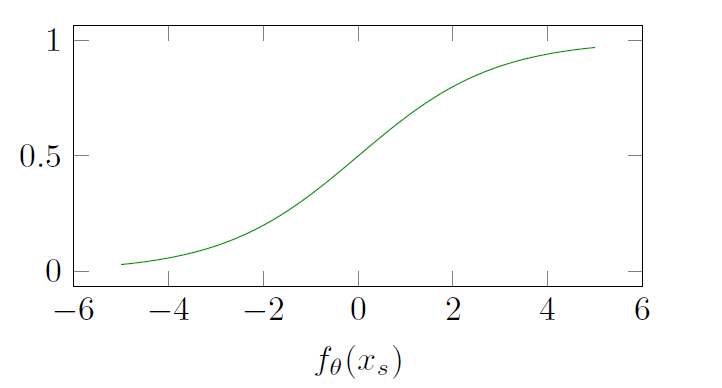
\includegraphics[width=.4\textwidth]{./resources/log_res.png}}
\subfigure[$\forall v\in V: p_{\Theta_v}(\theta_v)=\frac{1}{\sigma\sqrt{2\pi}}e^{\frac{-\theta^2_v}{2\sigma^2}}$]{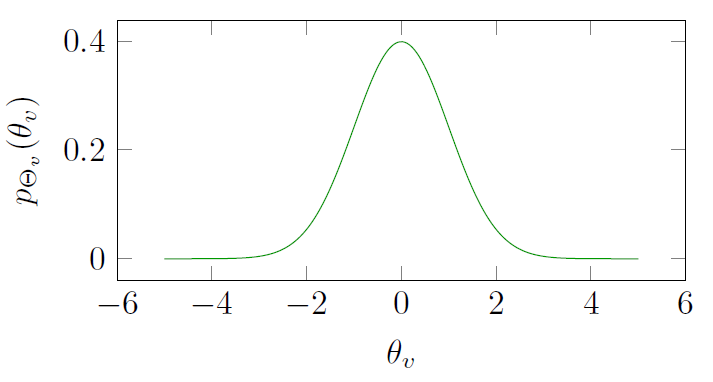
\includegraphics[width=.4\textwidth]{./resources/normal_dist.png}}
\end{figure}
Man kann nun Zeigen, dass das Finden der besten Parameter $\theta$, unter gegebenen Attributen x und Labeln y, äquivalent zum supervised learning Problem ist, sofern man die Lossfunktion, den Regularizer und $\lambda$ entsprechend wählt:\nl
\begin{itemize}
\item $\displaystyle\argmax_{\theta\in\mathbb{R}^m} p_{\Theta|X,Y}(\theta, x, y) \Leftrightarrow \displaystyle \inf_{\theta\in\Theta} \; \lambda R(\theta) + \frac{1}{|S|} \sum_{s\in S} L(f_\theta (x_s), y_s)$
\item wenn für L,R und $\lambda$ gilt:
\begin{itemize}
\item $\forall r\in \mathbb{R}\, \forall \hat{y}\in \{0,1\}: L(r, \hat{y}) = -\hat{y}r+\log(1+2^r)$
\item $\forall \theta\in \Theta: R(\theta) = \|\theta\|^2_2$
\item $\lambda = \frac{\log e}{2\sigma^2}$
\end{itemize}
\item Dieses Problem wir auch das \textbf{$\mathbf{l_2}$-regularized logistic regression problem} genannt (mit Bezug auf x, y, $\sigma$)
\end{itemize}
Beweis:
\begin{itemize}
\item $\displaystyle \argmax_{\theta\in\mathbb{R}^m} p_{\Theta|X,Y}(\theta, x, y)$
\item $\displaystyle =\; \argmax_{\theta\in\mathbb{R}^m} \prod_{s\in S} p_{Y_s|X_s,\Theta}(y_s,x_s,\theta)\prod_{v\in V} p_{\Theta_v}(\theta_v)$ 
\item $\displaystyle =\; \argmax_{\theta\in\mathbb{R}^m} \sum_{s\in S} \log\,p_{Y_s|X_s,\Theta}(y_s,x_s,\theta)+\sum_{v\in V} \log\,p_{\Theta_v}(\theta_v)$\\
gleich zur Zeile darüber, da der Logarithmus monoton ist und somit sich zwar der Wert des Maximums ändert, nicht aber die Stelle (arg), Umformung der Produkte in Summen mittels: $\log(x \cdot y) = \log(x) + \log(y)$
\item $\log p_{Y_s|X_s,\Theta}(y_s,x_s,\theta)$
\item $=\; y_s \log p_{Y_s|X_s,\Theta}(1,x_s,\theta) + (1-y_s)\log p_{Y_s|X_s,\Theta}(0,x_s,\theta)$\\
\red{Wie ? irgendwas mit gegenwsks ?}
\item $=\; y_s \log \frac{p_{Y_s|X_s,\Theta}(1,x_s,\theta)}{p_{Y_s|X_s,\Theta}(0,x_s,\theta)}+p_{Y_s|X_s,\Theta}(0,x_s,\theta)$\\
erhalten durch das Ausklammern von $y_s$, Anwendung von $\log (x) - \log (y) = \log \frac{x}{y}$
\item $\frac{p_{Y_s|X_s,\Theta}(1,x_s,\theta)}{p_{Y_s|X_s,\Theta}(0,x_s,\theta)}=\frac{\frac{1}{1+2^{-\langle x_s, \theta \rangle}}}{1-\frac{1}{1+2^{-\langle x_s, \theta \rangle}}}=\frac{1}{1+2^{-\langle x_s, \theta \rangle} -1}=2^{\langle x_s, \theta \rangle}$\\
Im Nenner ist das Gegenereignis vom Zähler, daher 1-..., da wir logistische Regression benutzen setzen wir hier die Formel dafür ein
\item $\displaystyle \argmin_{\theta \in \mathbb{R}^m} \sum_{s\in S} (-y_s \langle\theta,x_s\rangle + \log(1+2^{\langle \theta,x_s\rangle}))+\frac{\log e}{2\sigma^2}\|\theta\|^2_2$\\
\red{how ? detailed explain}
\end{itemize}
\subsection{Algorithmus}
Das $l_2$-regularized logistic regression problem kann mittel des \textbf{steepest descent Algorithmus} gelöst werden mit einem \textit{Toleranzparameter} $\epsilon \in \mathbb{R}^+_0$
\begin{itemize}
\item $\theta := 0$\\
initialisiere $\theta$
\item repeat:
\begin{itemize}
\item $d := \nabla \varphi(\theta)$\\
berechne die Schrittrichtung (Gradient)
\item $\displaystyle \eta := \argmin_{\eta'\in\mathbb{R}} \varphi(\theta - \eta'd)$ (line search)\\
Suche in Schrittrichtung d jene Schrittdistanz $\eta$ für welche der Loss+Regularizer am kleinsten ist
\item $\theta := \theta - \eta d$\\
gehe von $\theta$ in Richtung d um $\eta$ Einheiten, dort ist dann das neue $\theta$
\item if $\|d\| < \epsilon$\\
ist die gelaufene Strecke kleiner als unserer Toleranzparameter bricht ab, da wir uns nah genug am Minimum befinden
\begin{itemize}
\item return $\theta$
\end{itemize}
\end{itemize}	
\end{itemize}

\red{ToDO Letzter Beweis von linear function Kapitel}

\section{Semi-supervised / Unsupervised Learning}
\red{Details ergänzen}\\
Anderes als beim Supervised learning ist beim Semi/Unsupervised learning nicht jedem Sample ein Label zugeordnet, außerdem muss anderes als beim supervised learning auch nicht jede Labelzuodnung gültig sein. Darum verwenden wir im Weiteren eine Menge $\mathcal{Y} \subseteq \{0,1\}^S$ genannt \textbf{feasible labelings} für welche zudem gilt:
\begin{itemize}
\item $\mathcal{Y} = \{0,1\}$, Spezialfall entspricht unlabled data
\item $|\mathcal{Y}| = 1$, Spezialfall entspricht labled data
\item nicht-triviale (d.h. andere als die zwei Fälle oberhalb) erlaubt es endliche Strukturen zu kodieren, z.B. Maps, Äquivalenzrelationen oder Ordnungen
\end{itemize}

\subsection{learning und inference}
Sei folgendes gegeben:
\begin{itemize}
\item $T=(S,X,x,\mathcal{Y})$, constrained data
\item $\Theta \neq \emptyset$ mit $f: \Theta \rightarrow \mathbb{R}^X$
\item $R: \Theta \rightarrow \mathbb{R}^+_0$, Regularizer
\item $L:\mathbb{R}\times\{0,1\}\rightarrow\mathbb{R}^+_0$, Lossfunction
\item $\lambda\in\mathbb{R}^+_0$, regularizarion Parameter
\end{itemize}
Daraus lässt sich nun das \textbf{learning and inference Problem} definieren:\nl
$\displaystyle \min_{y\in\mathcal{Y}} \inf_{\theta\in\Theta}\; \lambda R(\theta) + \frac{1}{|S|}\sum_{s\in S} L(f_\theta (x_s), y_s)$\nl
Den Spezialfall wenn $\mathcal{Y} = \{\hat{y}\}$ nennt man \textbf{supervised learning problem}. Den Spezialfall wenn $\Theta = \{\hat{\theta}\}$ nennt man \textbf{inference problem}, dieses kann wie folgt formuliert werden:\nl
$\displaystyle \min_{y\in\mathcal{Y}}\; \sum_{s\in S} L(f_{\hat{\theta}} (x_s),y_s)$

Dieses inference Problem kann in ein binäres lineares Optimierungsproblem umgewandelt werden:
\begin{itemize}
\item $\displaystyle \argmin_{y\in\mathcal{Y}} \sum_{s\in S} L(f_{\hat{\theta}} (x_s),y_s)$
\item $\displaystyle = \; \argmin_{y\in\mathcal{Y}} \sum_{s\in S} y_s L(f_{\hat{\theta}} (x_s),1) + (1-y_s) L(f_{\hat{\theta}} (x_s),0)$
\item $\displaystyle = \; \argmin_{y\in\mathcal{Y}} \sum_{s\in S} y_s (L(f_{\hat{\theta}} (x_s),1) - L(f_{\hat{\theta}} (x_s),0)$
\end{itemize}

\section{Klassifizierung}
Bei der Klassifizierung versuchen wir eine Abbildung $\varphi$ zu finden, welche Elemente einer Menge A exakt ein \textbf{Klassenlabel} aus einer Menge B zuweist, d.h. $\varphi: A\rightarrow B$\\

\subsection{Formal}
Suche jene $\varphi: A\rightarrow B$ aus $\varphi \subseteq	A \times B$ für die gilt:
\begin{itemize}
\item $\forall a\in A \, \exists b\in B: (a,b) \in \varphi$\\
Jedes Element aus A muss ein Klassenlabel erhalten
\item $\forall a\in A, \, \exists b,b' \in B: (a,b) \in \varphi \land (a,b')\in\varphi \Rightarrow b=b'$\\
Jedes Element aus A hat exakt ein Klassenlabel
\end{itemize}
für diese Abbildung gilt somit auch:\nl
$\displaystyle \forall a\in A: \sum_{b\in B} y_{ab} = 1$,\nl
d.h. die Zuweisungsflag y ist genau einmal 1, also wird nur genau ein Klassenlabel zugewiesen, $y(a,b) = 1$ bedeutet dabei nicht, dass die Klassifikation von a als b korrekt ist, sondern lediglich, dass die gelernte Funktion a als b klassifiziert\nl
Wir betrachten bei der Klassifizierung \textbf{constrained data} $(S,X,x,\mathcal{Y})$ mit:
\begin{itemize}
\item $S = A \times B$, Paare aus Elementen und Klassenlabeln
\item $X=B\times \mathbb{R}^V$, Class-Sampleattribute-pairs, s.d. das erste Element \textbf{immer} die Klasse ist\\
$\forall a \in A\, \forall b\in B \, \exists \hat{x} \in \mathbb{R}^V: x_{ab} = (b,\hat{x})$\\
z.B. x = (label, $atr_1$, $atr_2$, ...) -> Label wird immer am Anfang appended
\item $\displaystyle \mathcal{Y} = \big\{y\in \{0,1\}^S \, \big\vert \, \forall a \in A : \sum_{b\in B} y_{ab} = 1 \big\}$\\
jedes Sample wird zu genau einem Label gemappt
\end{itemize}
Wir nehmen uns nun eine \textbf{Menge linearer Funktionen mit separaten Koeffizienten}\nl
$\displaystyle \forall \theta\in\Theta \, \forall b\in B \, \forall \hat{x} in \mathbb{R}^V: f_\theta((b,\hat{x})) = \sum_{v\in V} \theta_{bv} \hat{x}_v = \langle \theta_b, \hat{x}\rangle$\nl
Aus dieser Funktionsschar wählen wir uns dann mittels des Klassenlabels b die benötigte Funktion aus. Z.B. gäbe es bei der Klassifizierung von handschriftlichen Ziffern 10 verschiedene Funktionen\nl

Seien folgende Zufallsvariablen gegeben:
\begin{itemize}
\item $X_{ab}$, Attributsvektor
\item $Y_{ab}$, Decisionflag
\item $\theta_{bv}$, Parameter
\item $\mathcal{Z}\subseteq \{0,1\}^{A\times B}$, feasible descisions (wir suchen $\mathcal{Z} = \mathcal{Y}$)
\end{itemize}
Für diese ZF's lassen sich dann wieder Supervised Learning $P(\Theta|X,Y,Z)$ und Inference $P(Y|X,Z,\theta)$ formulieren\nl
Die ZF's sind dabei für $P(Y|X)$ logistisch verteilt, für die Parameter $\Theta$ normal verteilt und für $P(Z|Y$ gleich verteilt\nl
\textbf{uniform distribution}\\
$\displaystyle \forall \mathcal{Z} \{0,1\}^{A\times B} \, \forall y \in \{0,1\}^{A\times B}: p_{Z|Y}(\mathcal{Z},y) \propto \begin{cases} 1 & y\in \mathcal{Z}\\0 & \text{else} \end{cases}$
Man stellt fest, dass das Finden der besten Parameter $\theta$ unter Attributen x und Decisions y in $|B|$ separate unabhängige Teilprobleme aufgeteilt werden kann, diese können dann auch separat gelöst werden.\\
\textbf{Beweis}:
\begin{itemize}
\item $\displaystyle \argmax_{\theta \in \mathbb{R}^{B\times V}} p_{\Theta |X,Y,Z}(\theta,x,y,\mathcal{Y})$
\item $\displaystyle =\; \argmin_{\theta \in \mathbb{R}^{B\times V}} \; \sum_{(a,b)\in A\times B} (-y_{ab} f_\theta(x_{ab}) + \log (1+2^{f_\theta(x_{ab})}))+ \frac{\log e}{2\sigma^2} \| \theta \|^2_2$\\
flipping sign macht aus max ein min, einsetzen der Formel für Supervised learning, dort dann einsetzen von normal und log. distribution, aus Produkt mach Summe mit Logarithmus
\item $\displaystyle \min_{\theta \in \mathbb{R}^{B\times V}} \; \sum_{(a,b)\in A\times B} (-y_{ab} \langle \theta_b, x'_{ab} \rangle + \log (1+2^{\langle \theta_b, x'_{ab} \rangle}))+ \frac{\log e}{2\sigma^2} \| \theta \|^2_2$\\
einsetzen der weighted sum für $f_\theta$
\item $\displaystyle =\; \min_{\theta \in \mathbb{R}^{B\times V}} \;  \sum_{b\in B} \big(\sum_{a\in A}  (-y_{ab} \langle \theta_b, x'_{ab} \rangle + \log (1+2^{\langle \theta_b, x'_{ab} \rangle})) \big)+ \frac{\log e}{2\sigma^2} \| \theta \|^2_2$\\
aufteilen der Summe über Paaren in 2 Summen
\item $\displaystyle =\; \sum_{b\in B} \; \min_{\theta \in \mathbb{R}^{B\times V}} \;   \big(\sum_{a\in A}  (-y_{ab} \langle \theta_b, x'_{ab} \rangle + \log (1+2^{\langle \theta_b, x'_{ab} \rangle})) \big)+ \frac{\log e}{2\sigma^2} \| \theta \|^2_2$\\
\red{rausziehen der Summe da konstant ???}
\end{itemize}
Für jede constrained data, Parameter, und Descision gibt es eine Lösung für das Inference Problem, wenn bestimmte Bedingungen gelten:
\begin{itemize}
\item $\displaystyle \min_{y\in \mathcal{Y}} \; \sum_{(a,b)\in A\times}  L(f_\theta(x_{ab}),y_{ab})$ hat eine Lösung wenn:
\begin{itemize}
\item $\displaystyle \forall a \in A: \varphi(a) \in \max_{b\in B} \langle \theta_b,x'_{ab} \rangle$, jedes Element bekommt irgendein Label zugeordnet (aus den Maximas der Funktionsschar)
\item $\forall (a,b)\in A \times B: \hat{y}_{a} = 1 \Leftrightarrow \varphi(a) = b$, Wenn das Klassenlabel b dem Element a zugeordnet wurde so muss das Mapping das gleiche Ergebnis repräsentieren
\end{itemize}
\end{itemize}
\textbf{Beweis}:
\begin{itemize}
\item \red{Todo}
\end{itemize}

\section{Wahrscheinlichkeit}
\subsection{Example 1}
Seien $A$ und $B$ zwei Würfel und sei $X=A+B$ die Summe beider Würfel
\begin{itemize}
\item $P(A=2,B=3,X=7) = 0$, da es unmöglich ist, das alle 3 sich im angegebenen Zustand befinden
\item $P(A=2,B=3,X=5) = \frac{1}{36}$, genau 1 Ereignis (von 36) erfüllt alle Zustände
\item $P(X=5|A=2, B=3) = 1$, die Wsk. dass $A+B =5$ wenn wir wissen, das $A=2$ und $B=3$ ist natürlich 1
\item $P(A,B|X=5) = \frac{1}{4}$, es gibt nur 4 verschiedene Kombinationen von $A$ und $B$, s.d. $A+B=5$\\
$X=A+B \rightarrow 5=1+4=2+3=3+2=4+1$
\end{itemize}
\subsection{Example 2}
\begin{itemize}
\item $P(B|A)=\frac{P(A,B)}{P(A)}=\frac{P(A,B)}{\sum P(A,B)}$
\item $P(A,B)=P(A|B)P(B)$
\item $P(A,B)=P(A\cup B)$
\item $P(A,B,C) = P(A|B,C)P(B,C)=P(A|B,C)P(B|C)P(C)$
\end{itemize}



\end{document}